\section{Weather Analysis}
\label{sec:analysis}

% Opening {{{

In this section, we use our collected data to understand how
weather conditions affect dropouts. 

% }}}

\if 0
\subsection{Categorical weather} % {{{

First, we investigate weather conditions for which a Boolean value can be determined using weather records. Weather records contain aw and mw values which specify special weather conditions, such as thunderstorm, rain, snow, hail etc.  

% \begin{figure*}[tb]
% \centering
% \includegraphics[width=0.32\linewidth]{figs/comp_frate_by_timeofweek_CABLE_iststormvsall_jan11todec17_ci_whiskers}
% \includegraphics[width=0.32\linewidth]{figs/comp_frate_by_timeofweek_CABLE_israinvsall_jan11todec17_ci_whiskers}
% \includegraphics[width=0.32\linewidth]{figs/comp_frate_by_timeofweek_CABLE_issnowvsall_jan11todec17_ci_whiskers}
% \caption{
% \label{fig:discretefrate_timeofweek} For Cable addresses, more
% addresses are likely to become unresponsive during rain and
% thunderstorm during most hours of the week, including hours when there
% are higher baseline responsive to unresponsive transitions.}
% \end{figure*}

% Figure~\ref{fig:discretefrate_timeofweek} shows responsive to
% unresponsive transitions during the hours of the week for
% thunderstorm, rain, and snow. 

% }}}
\fi

\subsection{Relative dropout rates} % {{{
\label{sec:inflations}


% Inflated dropout rates, histogram {{{

\begin{figure*}[t]
\centering
\includegraphics[width=\linewidth]{weather/figs/inflatedfrate_by_wtyp_ci_whiskers}
\caption{
\label{fig:inflatedfrate_by_wtyp_ci_whiskers}
\figdone
	The number of response-hours (in centuries) for which we have measured various link
	types in various weather conditions (top), and the additional
	(``inflated'') probability of dropout experienced in those link-
	and weather-types (bottom).}
\end{figure*}

% }}}

First, we analyze the relative rate of dropouts under various link types
and weather conditions, after omitting all hurricane periods.
%
We use categorical data from 
weather records (such as ``thunderstorm present''),  to assign a
single weather condition for each hour. 
% 
If more than one weather condition occurred in an hour, then we assign
the most severe condition to that hour.
% 

%
The top of Figure~\ref{fig:inflatedfrate_by_wtyp_ci_whiskers} shows the
number of responsive hours for which we measured the various link- and
weather-types.
%
Although there is a wide range in their absolute values (note the
log-scale of the $y$-axis), the overall shape of the histograms remains
mostly consistent across the different link types.
%
This reflects the fact that, in their deployment throughout the US,
different link types are exposed to very similar conditions, with one
minor exception: we did not measure any fiber or satellite links during
tornadoes.


The bottom of Figure~\ref{fig:inflatedfrate_by_wtyp_ci_whiskers} shows
the difference in the probability of failure rate between the presence
of a weather condition and its absence.
%
A value of zero signifies no observed difference with or without a
particular weather condition; positive values indicate increased
probability of dropout during that weather condition; and negative
values indicate \emph{fewer} failures during that weather condition.
%
In the bottom of the figure, we also include confidence intervals on
all bars; they are tight on almost all values, but satellite links are
noticeably variable, as are tornadoes.


We make three key observations from
Figure~\ref{fig:inflatedfrate_by_wtyp_ci_whiskers}.
%
First, there are several weather conditions that exhibit higher dropout
probabilities across \emph{all} of the link types we measured.
%
Thunderstorms, heavy rain, moderate rain, and (for the link types that
experienced it) tornadoes all yield a statistically significant
increase in dropout probabilities.


Second, for each given link type, heavier rates of precipitation (both
rain and snow) yield higher probabilities of dropout.
%
We analyze dropout rates as a function of precipitation in
Section~\ref{sec:continuous}.
%
Interestingly, the probability of dropouts is greater during
thunderstorms than during heavy rain for all link types.
%
Recall that we classify ``thunderstorm'' and ``heavy rain'' as mutually
exclusive.
%
This indicates that the causes of failures during thunderstorms extend
beyond the rainfall, perhaps to increased wind or power outages.
%
%% We evaluate the combined effects of precipitation and wind speed in
%% Section~\todo{ref}.


% Inflation by state {{{

\begin{figure*}[t]
\centering
\includegraphics[width=\linewidth]{weather/figs/inflatedfrate_ALL_by_state_pcpexcl}
\caption{\label{fig:inflatedfrate_by_state_pcp}
\figdone
Top: Inflation in hourly dropout probability by U.S.~state for thunderstorm, rain, and
	snow (with 95\% confidence intervals). Bottom: The fraction of link
	types by U.S.~state (the remaining fraction are of unknown type).
	}
\end{figure*}

% }}}

% US Maps {{{
\begin{figure*}[t]
\begin{subfigure}[t]{0.32\linewidth}
\centering
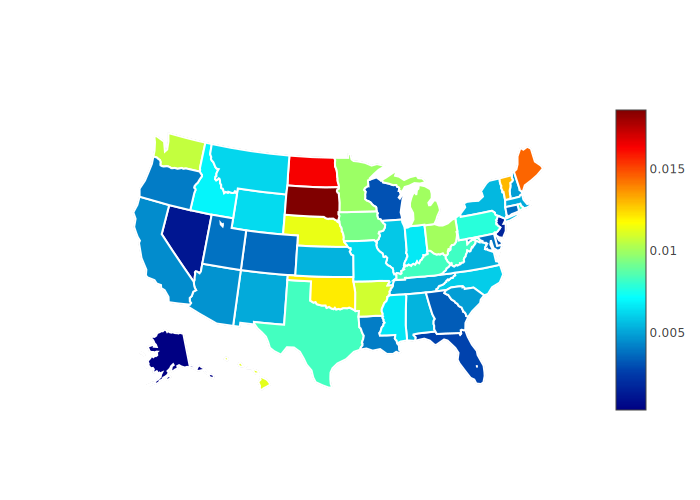
\includegraphics[width=\linewidth]{weather/figs/normalizedfratebyexclweather_ALL_iststorm_statewise_jan11todec17_heatmap}
\caption{
\label{fig:inflatedfrate_tstorm_usmap}
Thunderstorm
}
\end{subfigure}
%
\begin{subfigure}[t]{0.32\linewidth}
\centering
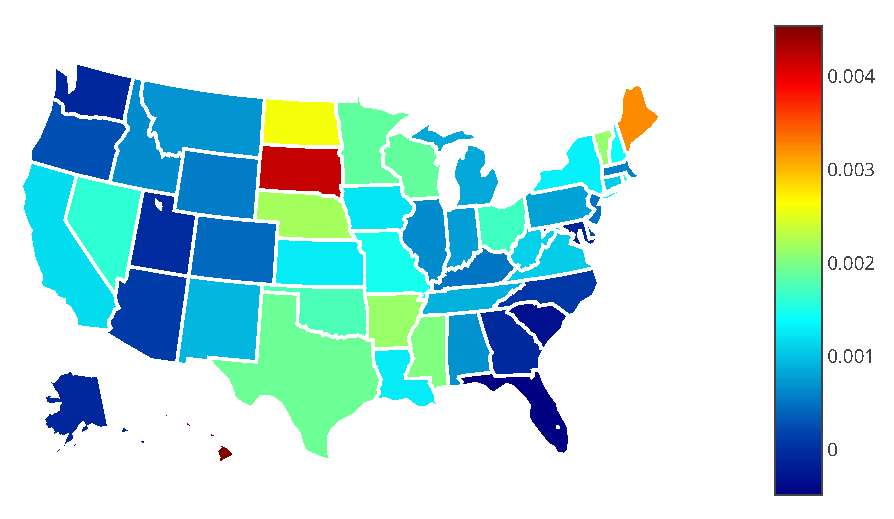
\includegraphics[width=\linewidth]{weather/figs/normalizedfratebyexclweather_ALL_israin_statewise_jan11todec17_heatmap}
\caption{
\label{fig:inflatedfrate_rain_usmap}
	Rain}
\end{subfigure}
%
\begin{subfigure}[t]{0.32\linewidth}
\centering
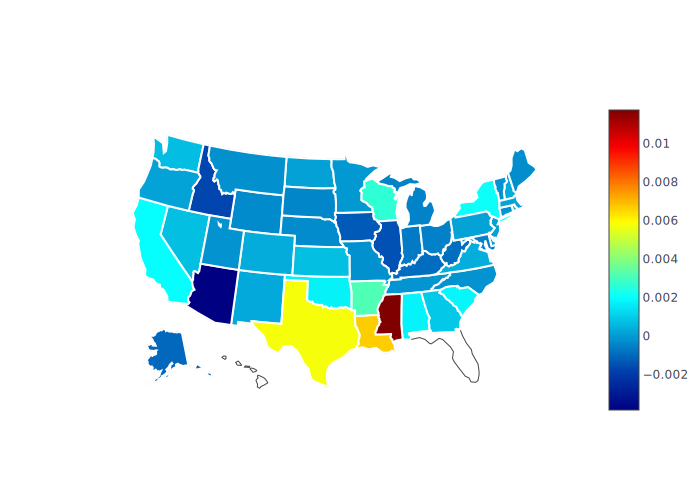
\includegraphics[width=\linewidth]{weather/figs/normalizedfratebyexclweather_ALL_issnow_statewise_jan11todec17_heatmap}
\caption{
\label{fig:inflatedfrate_snow_usmap}
	Snow}
\end{subfigure}
%
\caption{
\label{fig:inflatedfrate_maps}
\figdone
Inflation in hourly dropout probability by U.S.~state for various
	weather conditions.  Large geographic regions can exhibit common
	behavior; northern states are more prone to failures in
	thunderstorms, Midwestern states in rain, and southern states in
	snow.  (Note the different scales for each sub-figure.)}
\end{figure*}
% }}}


Finally, the dropout probabilities of wired link types (cable, DSL, and
fiber) are similar to one another, as are the dropout probabilities of
wireless link types (WISP and satellite), but wired and wireless link
types are different from one another.
%
For example, light rain and light snow have almost no discernible
difference in dropout probabilities for wired links, but light rain
exhibits higher dropout probability for wireless links, and light snow
sees \emph{lower} probability of dropout.
%
Conversely, gale-force winds have a profound increase in dropout
probabilities for wired links, but wireless links are less likely to
drop out during them.
%
It is not surprising that strong winds can cause wired links to fail,
for instance by knocking down above-ground cables.
%
Although wireless links are not affected in the same way, it is
surprising that higher failure rates would not be observed, given that
such strong winds could destroy or blow away satellite dishes.


\paragraph{Summary and ramifications}
%
The results from Figure~\ref{fig:inflatedfrate_by_wtyp_ci_whiskers}
collectively show that different link types can experience weather in
different ways.
%
It is not surprising that different link types would differ in the
\emph{magnitude} with which they experience dropouts; but what we do
find surprising is that some weather conditions (especially snow and
cold) can differ in whether they increase or \emph{decrease} dropout
rates.
%
This has ramifications on network measurement methodology: when
performing outage analysis, it is important to account for both link
type \emph{and} weather condition.
%
%% In the results that follow, we delve deeper into these dropouts by
%% exploring whether dropouts vary across fine-grained measures of wind
%% speed and precipitation, and whether there are geographic influences on
%% weather's effect.




% }}}

\subsection{Geographic variation} % {{{
\label{sec:geography}

Next, we investigate the extent to which different geographic regions
experience weather in different ways.
%
Of course, different states experience different \emph{amounts} of
weather (for instance, we did not observe a statistically significant
amount of snow in Florida).
%
To control for this, we present the inflated probability of hourly
dropouts, comparing hours with a particular weather condition (e.g.,
snow) against all hours without that weather condition.
%
This gives us an apples-to-apples comparison across states, even if
they experience weather conditions in varying amounts.

In Figure~\ref{fig:inflatedfrate_by_state_pcp}, we present the dropout
probability inflation across all 50 U.S.~states (and DC) for three weather
conditions: thunderstorms, rain (excluding hurricanes), and snow.
%
We make two key observations.
%
First, there is a high variation of increased dropout probability across states.
%
For example, during thunderstorms, South Dakota experiences an average
increased hourly dropout probability of 0.018 (3.1 additional
failures per week), while New Jersey increases by only 0.0038 (2.9
additional failures per \emph{month}).
%
Moreover, as shown by the 95\% confidence intervals in the figure,
these differences are statistically significant.
%
We believe this to be an important result because it shows
the role that geography plays in network outages. 


Second, while the raw dropout inflation varies among states, the
relative impact of weather types is common across \emph{most} states:
the increase in dropouts during thunderstorms tends to be greater than
in rain, which in turn tends to be greater than in snow.
%
There are a few notable exceptions.
%
Louisiana and Mississippi have more inflated dropouts in snow than in
thunderstorms, and Florida tends to experience similar amounts of
failures in rain as it does in thunderstorms.
%
By controlling for geography and the total amount of time spent in
weather, this result shows that some weather conditions have more
pronounced impact on dropouts.

Below Figure~\ref{fig:inflatedfrate_by_state_pcp}, we
present a breakdown of the classified link types in each
state, weighted by responsive hours in probing.  The intent
of consulting this graph is to determine whether the outliers
in the top graph are a direct function of the link types  that
are prevalent in a state. North
Dakota has a substantial and exceptional deployment of
Fiber: 50\% of the link-type-classified responsive hours are
from Fiber addresses.  Although our sampling approach is
based on finding 100 addresses in each provider in a region,
and thus is not meant to sample the distribution of link
types used by customers, we note that this is consistent
with published reports that ``60 percent of the households,
including those on farms in far-flung areas, have
fiber''~\cite{csgmidwest}.  Although there are instances where
top and bottom graphs appear related---Vermont (VT) and Maine (ME) show both a
high vulnerability to thunderstorms and a relatively large proportion
of DSL compared to immediate neighbors CT, NH, MA---it appears that
geography is more important than link type at determining the
inflation in probability of dropout in precipitation.




Next, we look beyond individual states to see if there are
\emph{regional} correlations of dropouts.
%
In Figure~\ref{fig:inflatedfrate_maps}, we show maps with the average
inflation in dropout probabilities during thunderstorms, rain
(excluding hurricanes), and snow.


During thunderstorms (Figure~\ref{fig:inflatedfrate_tstorm_usmap}) and
rain (Figure~\ref{fig:inflatedfrate_rain_usmap}) Midwestern states tend
to experience greater inflation of dropouts than other regions.
%
(Maine is an outlier; its dropout inflation during thunderstorm and
rain is due to an abnormally powerful series of storms in
October~2017.)
%
Recall from Figure~\ref{fig:inflatedfrate_by_wtyp_ci_whiskers} that
WISP and satellite links fail more often in thunderstorms and rain than
other link types.
%
One possible explanation for higher dropout rates in the Midwest would
be that these states have more wireless links.
%
This hypothesis is confirmed in
Figure~\ref{fig:inflatedfrate_by_wtyp_ci_whiskers}, which shows that
Midwestern states have more satellite links than other states.


During snow (Figure~\ref{fig:inflatedfrate_snow_usmap}), we see more
pronounced dropout inflation in southern states.\footnote{We do not
include data for Florida or Hawaii, as we did not
observe enough responsive hours of snow to achieve statistical
significance.}
%
Texas, Louisiana, and Mississippi experienced drastically higher
probability of dropouts in snow than in the absence of snow.
%
Unlike rain and thunderstorm, this disparity cannot be explained by
link type alone, as no link types experience drastically higher dropout
rates than others (in fact,
Figure~\ref{fig:inflatedfrate_by_wtyp_ci_whiskers} shows that wireless
links tend to experience \emph{fewer} dropouts during snow).
%
Our insight is that snow seems to affect states where snow is less
common.



% Commonality vs severity plots {{{


% \begin{omitfigure}
% \begin{figure}[t]
% \centering
% \includegraphics[width=\linewidth]{weather/figs/numweatherhours_vs_frate_snow_scatter}
% \caption{
% \label{fig:numweatherhours_vs_frate_snow_scatter}
% P(Dropout) per U.S. state vs. hours of received snow}
% \end{figure}
% \end{omitfigure}

% TODO TODO TODO: Fix this.
% \begin{figure}[t]
% \centering
% \includegraphics[width=0.7\linewidth]{weather/figs/numweathers_vs_frate_snow_scatter}
% \caption{
% \label{fig:numweathers_vs_frate_snow_scatter}
% \figdone
% 	Hourly dropout probability of hosts (all link types) as a function
% 	of the number of hours the hosts' nearest U.S.~airport received
% 	snow (truncated to only those with fewer than 100 hours in snow).
% 	The less common snow is in a region, the more impact it tends to
% 	have.}
% \end{figure}


% \begin{omitfigure}
% \begin{figure}[t]
% \centering
% \includegraphics[width=\linewidth]{weather/figs/numweathers_vs_frate_rain_scatter}
% \caption{
% \label{fig:numweathers_vs_frate_rain_scatter}
% P(Dropout) per U.S. state vs. proportion of hours of received rain}
% \end{figure}

% \begin{figure}[t]
% \centering
% \includegraphics[width=\linewidth]{weather/figs/numweathers_vs_frate_tstorm_scatter}
% \caption{
% \label{fig:numweathers_vs_frate_tstorm_scatter}
% P(Dropout) per U.S. state vs. proportion of hours of received tstorm}
% \end{figure}
% \end{omitfigure}

% }}}

One possible explanation for the regional effects is therefore that
regions that are less ``familiar'' with a particular weather condition
may be more heavily affected by it.
%
To evaluate this hypothesis, we plot in
Figure~\ref{fig:numweathers_vs_frate_snow_scatter} the hourly dropout
rate of each U.S.~airport as a function of the number of hours each
airport has spent in snow.
%
The results in this figure confirm our hypothesis for snow: the less
familiar a location is to snow, the more often it tends to experience
dropouts.
%
Areas with very small amounts of snow do not experience large
inflation  (ostensibly because there is not enough time for it to
cause damage).
%
Conversely, areas with snow beyond a threshold are more resilient to
snow.
%
A likely reason for this is that regions that are more used to snow
tend to invest more in infrastructure to prepare for and mitigate
it~\cite{state-dots-snow-spending}.
%
We also performed this analysis under thunderstorms and rain (figures
not shown), but did not observe as strong an effect.
%
We hypothesize that this is because all of the airports we measured
experienced enough thunderstorm and rain to grow accustomed to them.

\paragraph{Summary and ramifications}
%
We conclude from these results that different geographic regions can be
affected by weather to varying degrees.
%
We attribute this geographic variation to two leading factors: (1)~the
predominance of some link types over others (e.g., wireless links are
more common in the Midwest), and (2)~how familiar a region is with a
particular weather condition (and thus how prepared for it the region
is).
%
Our results have several interesting ramifications on outage analysis.
%
First, when performing outage analysis, it is important to consider a
representative set of locations and link types; measuring only, say,
cable links would risk overestimating the Midwest's resilience to
dropouts.
%
Second, it is important to note the time and weather conditions when
outage measurements are taken; collecting measurements only during
Spring months\footnote{For instance, in the run-up to the IMC
deadline.}, when thunderstorms are more common, would risk
overestimating dropouts year-round.



% }}}

\subsection{Continuous weather variables} % {{{
\label{sec:continuous}

Thus far in our analysis, we have considered various \emph{binary}
classifications of weather---rain (or not), snow (or not), gale (or
not), and so on.
%
Although these classifications are standard (they are included in the
weather reports we collect), they risk masking the precise effect that
various weather conditions can have.
%
Here, we evaluate dropouts as a function of several \emph{continuous}
weather variables: wind speed, precipitation, and temperature.


Figure~\ref{fig:wind_cont} shows the inflation in the hourly dropout
probability of various link types as a function of wind speed.
%
Note that not all link types share the same values on the $x$-axis;
we aggregate data in increasing values of $x$ until we reach either an
interval of 10 mph or 20 dropout samples (Eq.~(\ref{eq:samples})), whichever comes last.


For all link types, we see almost no inflation in dropout probability
when wind speed is less than 30 mph.
%
Beyond 30 mph, there is little effect on wireless links (WISP and
satellite), but significant increases in dropout probability for wired
links: cable, DSL, and fiber.
%
This is reflected in
Figure~\ref{fig:inflatedfrate_by_wtyp_ci_whiskers}, which showed that
wireless links were not as affected by gale winds.
%
Figure~\ref{fig:wind_cont} expands on this by showing that, as wind speed
increases, dropout inflation increases at a super-linear rate---between
40~mph and 55~mph winds, Cable links' dropout inflation increases by an
hour of magnitude.


In Figure~\ref{fig:temp_cont}, we show dropout inflation as a function
of temperature.
%
Like with wind speed, we bin along the $x$-axis in units of 10, or
20 dropout samples, whichever comes second, and include 95\% confidence
intervals.
%
There are several surprising observations in this figure.
%
First, satellite links are highly sensitive to temperature; at low
temperatures, satellite links are far less likely to experience
dropouts, but this increases steadily, until at approximately
70$^\circ$\,F when satellite links become more likely to fail.
%
Surprisingly, at approximately 80$^\circ$\,F, there is an inflection point at
which satellite links again become significantly more reliable.
%
We hypothesize that there is a confounding factor: satellite links are
less reliable when there is no line-of-sight visibility (e.g., due to
fog), and we suspect that higher temperatures result in less fog.


\begin{figure}[t]
\centering
\includegraphics[width=0.7\linewidth]{weather/figs/inflatedfrateperbinnedval_wind_jan11todec17}
\caption{
\label{fig:wind_cont}
\figdone
Inflation in hourly dropout probability as a function of wind speed
	across multiple link types. All link types experience greater
	dropout probabilities, but satellite and WISP links increase the
	least.  }
\end{figure}

All of the other link types we measured exhibit similar behavior to one
another.
%
They have highly variable dropout probabilities at low temperatures;
they remain mostly steady until 60$^\circ$\,F, then they increase slightly with
higher temperatures.
%
Unlike with our other results, WISPs more closely resemble wired links
than satellite links; we hypothesize that this, too, is because
satellite links are affected by line-of-sight while WISPs and wired
links are not.


Finally, in Figure~\ref{fig:pcp_cont} we measure various link types'
dropout inflation as a function of precipitation in thunderstorms,
rain, and snow.
%
All link types exhibit increased dropout inflation with increased
precipitation, regardless of the overarching weather condition.
%
However, surprisingly, the magnitude of increase varies significantly
across link types.
%
Again, satellite tends to be the most sensitive to change.
%
Other link types are not as consistent across different types of
precipitation; WISP links exhibit nearly the same increase in dropouts
at high thunderstorm precipitation as satellite, but far less during
non-thunderstorm rain.
%
Similarly, DSL links experience a (varying but statistically
significant) increase in dropouts during high snow precipitation, but
not nearly as much during thunderstorm or rain.


There appears to be an inflection point with snow and rain: prior to
0.1~inches of precipitation in rain or snow, non-satellite links
experience little change in their dropout probabilities.
%
After these points, they increase significantly and quickly.
%
Conversely, most links experience (slight but statistically significant)
increases in dropout rates in all levels of precipitation during
thunderstorms.



\paragraph{Summary and ramifications}
%
Weather conditions are often described with binary categories: rain (or
not), snow (or not), and so on.
%
These continuous variable results show that such categories can be
overly coarse; the mere presence of rain or snow does not necessarily
affect most link types, unless there is more than 0.1~inches of
precipitation.
%
Like with our prior results, different link types can exhibit widely
varying behaviors, lending further motivation to incorporate link types
into future outage analyses.


%% Here, we consider continuous weather
%% variables such as rain, temperature, and wind speed.  Each point represents, at
%% some weather condition (x-axis value), how many outage-hours were seen divided
%% by the total number of hours (outage and non-outage) with that weather
%% condition. Where there are not at least 10,000 samples at an x value,
%% subsequent x-axis values are aggregated to determine the probability of failure
%% (y-axis position) and the midpoint between starting and ending x-axis values
%% used to determine the x-axis value.  Points appear for each link type; a line
%% appears for the aggregate of all observations: this line often tracks the DSL
%% points because a majority of our hosts are DSL attached.


% \begin{figure}[t]
% \centering
% \includegraphics[width=\linewidth]{figs/inflatedfrateperbinnedval_pcptstormrain_jan11todec17}
% \caption{
% \label{fig:rain_tstorm_cont}
% Precipitation in rain and thunderstorm}
% \end{figure}

\begin{figure}[t]
\centering
\includegraphics[width=0.7\linewidth]{weather/figs/inflatedfrateperbinnedval_temp_jan11todec17}
\caption{
\label{fig:temp_cont}
\figdone
Inflation in hourly dropout probability as a function of temperature 
	across multiple link types. All link types exhibit non-monotonic
	effects, typically increasing at higher and lower temperatures
	(satellite being a clear exception).
	%whereas most link types experience most failures in very
	% cold or very hot temperatures, 
	% satellite links are most affected in moderate temperatures
	% (70--90$^\circ$~F).
}
\end{figure}

\newlength{\triplefigwidth}
\setlength{\triplefigwidth}{2.3in}
\begin{figure*}[t]
\centering
% \includegraphics[width=\triplefigwidth]{weather/figs/inflatedfrateperbinnedval_pcptstorm_jan11todec17}%
\includegraphics[width=0.32\linewidth]{weather/figs/inflatedfrateperbinnedval_pcptstorm_jan11todec17}%
%
\hfill
%
\includegraphics[width=0.32\linewidth]{weather/figs/inflatedfrateperbinnedval_pcprain_jan11todec17}%
%
\hfill
%
\includegraphics[width=0.32\linewidth]{weather/figs/inflatedfrateperbinnedval_pcpsnow_jan11todec17}
\caption{
\label{fig:pcp_cont} Inflation in hourly dropout probability as a
	function of precipitation during thunderstorm (left), rain
	(center), and snow (right), across multiple link types. All link
	types experience higher dropout probabilities with more
	precipitation, but to widely varying magnitudes. (Note the
	different ranges of the $x$-axes.)}
\end{figure*}


% }}}
